LTE (Long Term Evolution) è la quarta generazione di reti mobili.
Il sistema è stato riprogettato in modo da abbracciare il paradigma "all-IP", dunque il piano di controllo e il piano utente sono basati su IP e la commutazione di circuito non è più supportata.
Viene inoltre introdotto il concetto di \textbf{flat network}, ovvero la rete di accesso radio include un singolo nodo, chiamato eNodeB.
Il piano dati e di controllo vengono separati, in modo che quello dati sia gestito in modo da attraversare il minor numero di nodi possibile.
Per aumentare le prestazioni sono stati fatti dei miglioramenti significativi al livello fisico, tra cui Multi-carrier modulation (OFDM/OFDMA), adaptive modulation e coding,
sistemi di antenne Multiple Input Multiple Output (MIMO).
\section{Architettura}
\begin{figure}[H]
	\centering
	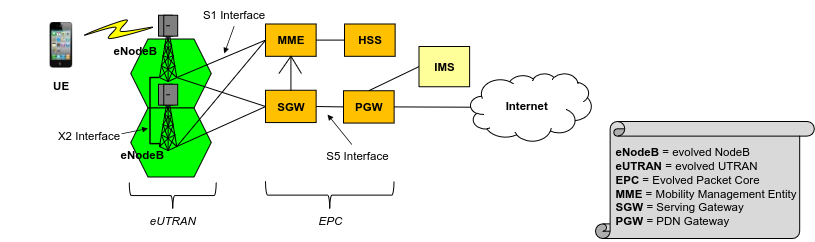
\includegraphics[width=\textwidth]{pictures/11/architettura.png}
	\caption{Architettura di rete LTE}
\end{figure}
La rete di accesso ora viene chiamata Evolved UTRAN (E-UTRAN). Tutti i servizi, inclusi quelli telefonici (VoLTE, con l'aiuto di IMS) vengono realizzati tramite IP.
Ora vediamo i componenti della rete:
\begin{itemize}
	\item \textbf{eNodeB}: base station evoluta, offre funzionalità estese.
	\item \textbf{Packet Data Network Gateway (PGW)}: connette le UE alle reti esterne (entry e exit point per il traffico dati).
	\item \textbf{Serving Gateway (SGW)}: instrada e inolta i pacchetti dati degli utenti.
	\item \textbf{Mobility Management Entity (MME)}: nodo principale del piano di controllo.
\end{itemize}
\begin{figure}[H]
	\centering
	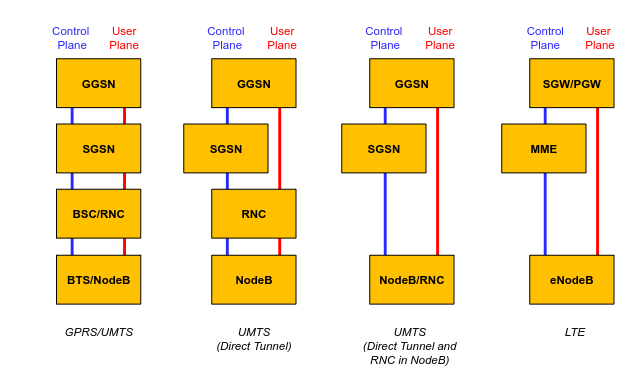
\includegraphics[width=0.9\textwidth]{pictures/11/evoluzioneFlat.png}
	\caption{Evoluzione delle reti mobili verso un'architettura flat}
\end{figure}
\begin{figure}[H]
	\centering
	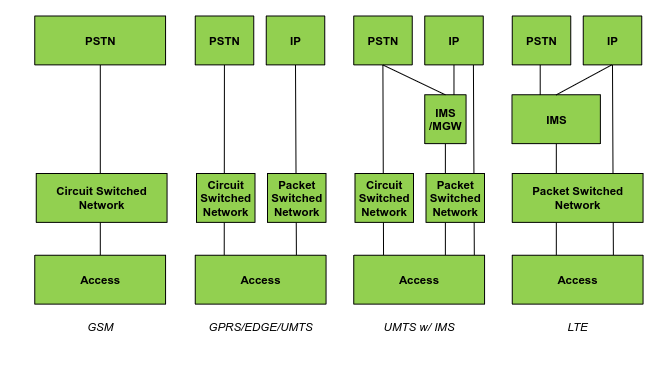
\includegraphics[width=0.9\textwidth]{pictures/11/evoluzioneAllIP.png}
	\caption{Evoluzione delle reti mobili verso un'architettura all-IP}
\end{figure}
\subsection{Miglioramenti}
I miglioramenti apportati alla core network sono importanti tanto quelli apportati alla RAN.
Le funzionalità del NodeB e RNC sono state collassate nel eNodeB.
Viene definita una nuova interfaccia X2, che permette il collegamento diretto tra eNodeB.
La latenza viene ridotta dai 50/100 ms di HSPA a 10 ms, principalmente grazie ai principi di flat network.
In questo modo, il supporto per applicazioni real-time e VoIP è migliorato.
Il supporto alle chiamate vocali viene offerto tramite IMS in VoLTE, o tramite internet working con reti 2G/3G (Call Setup fallback).
\section{eUTRAN}
La gestione dell'handover e la coordinazione tra celle viene gestita in maniera autonoma dagli eNodeB tramite X2.
\subsection{User Equipment}
Gli UE non sono solo telefoni, ma anche tablet, laptop, dispositivi IoT, etc.
Come nelle reti precedenti, gli UE includono sia la SIM che il TE (Terminal Equipment), che è l'entità che si connette alla rete.
Possono opzionalmente includere dei client VoIP per VoLTE, e avere più antenne per supportare MIMO.
Tendenzialmente sono multi-standard (GSM, UMTS, LTE).
\subsection{eNodeB}
Base station evoluta che gestisce una o più celle. Gestisce le risorse radio e alcune funzionalità di mobilità.
Include le funzionalità che erano offerte da NodeB e RNC (ad esempio iniziare le procedure di handover) e trasmette i messaggi di paging originati da MME.
Agisce come un nodo di relay verso gli SGW, instradando i pacchetti del piano dati verso quelli corretti.
Può essere collegato a un insieme di MME e SGW, benché ogni UE è connesso a uno solo di questi nodi.
\section{Evolved Packet Core (EPC)}
Può servire tecnologie di rete di accesso eterogenee, come LTE, UMTS,GSM/EDGE (3GPP access) e Wi-Fi (non-3GPP access).
Fornisce mobilità (anche handover tra sistemi eterogenei) e instradamento dei pacchetti.
\subsection{Mobility Management Entity (MME)}
Si occupa dell'autenticazione e procedure di sicurezza sia per il piano di controllo che per quello dati, in questo viene aiutato da HSS (Home Subscriber Server).\\
Per quanto riguarda la gestione della mobilità:
\begin{itemize}
	\item è simile al VLR/MSC delle reti 2G/3G.
	\item Memorizza le informazioni riguardanti la Tracking Area (TA) in cui si trova l'UE.
	\item Gestisce le procedure di handover quando queste non vengono gestite dagli eNodeB tramite interfaccia X2.
\end{itemize}
Per quanto riguarda la connettività dei servizi:
\begin{itemize}
	\item Crea nuovi bearer per gli UE in base alle richieste di QoS.
\end{itemize}
Un MME può servire più SGW.
\subsection{Serving Gateway (SGW)}
Un bearer tra il SGW e eNodeB (S1 bearer) viene creato quando un UE è nello stato attivo.
Quando questo avviene, viene inoltre creato un bearer radio tra UE e eNodeB.
Il SGW gestisce l'S1 bearer ed è il responsabile dello switching in caso di mobilità, una volta ricevuto un messaggio di handover da MME.
Nel caso non ci sia un'interfaccia X2, il SGW è coinvolto nell'handover tra eNodeB, re-instradando opportunamente i pacchetti dati.
Quando un PGW manda i pacchetti a un UE in stato idle, il SGW li buffera e invia al MME una richiesta di iniziare la procedura di paging.
\subsection{PDN Gateway (PGW)}
Punto di accesso alla rete mobile per le reti esterne. Assegna gli indirizzi IP agli UE tramite DHCP.
Implementa le funzionalità per l'addebito in base ai servizi e calcola informazioni statistiche sul traffico.
\subsection{Home Subscriber Server (HSS)}
Implementa le funzionalità di HLR/AUC e HSS nelle reti 3G.
Le funzionalità di HLR e HSS vengono collassate in modo che gli UE multi-standard possano facilmente avere accesso a servizi 2G/3G e 4G.
\section{Forward dei pacchetti}
Il forward dei pacchetti IP in mobilità di tipo active è basato su GTP
\begin{figure}[H]
	\centering
	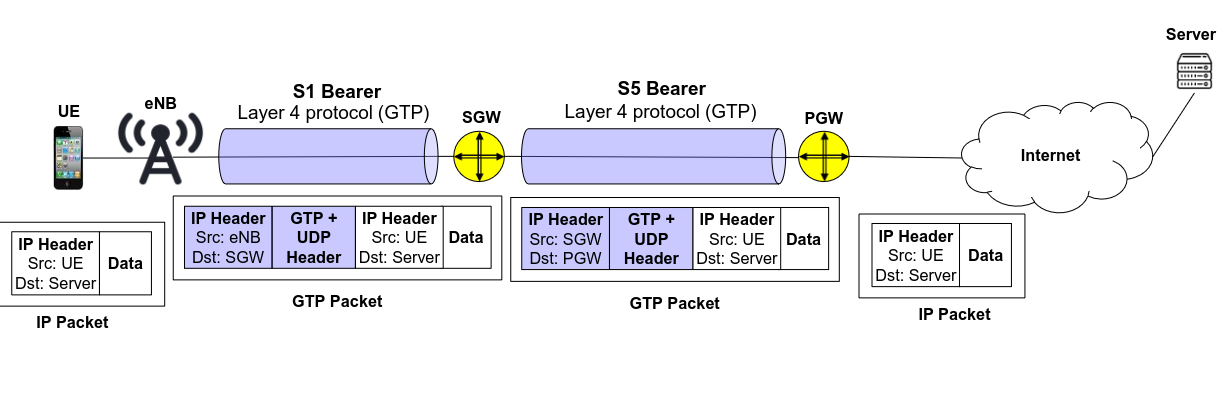
\includegraphics[width=\textwidth]{pictures/11/forward1.png}
\end{figure}
\begin{figure}[H]
	\centering
	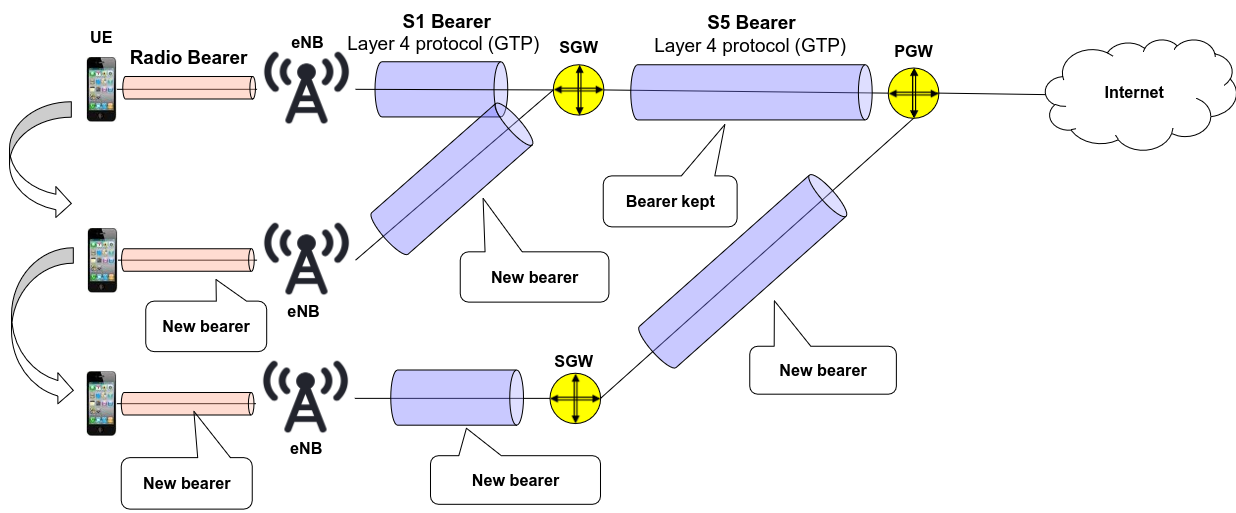
\includegraphics[width=\textwidth]{pictures/11/forward2.png}
	\caption{Forward dei pacchetti IP in mobilità di tipo active}
\end{figure}
\section{Procedure}
\subsection{Attach}
Un UE è localizzato tenendo traccia della Tracking Area presso la quale può essere raggiunto.
Quando un UE si accende, si attacca alla rete, effettuando la seguente procedura:
\begin{enumerate}
	\item Autenticazione mutuale
	\item Assegnazione di un indirizzo IP all'UE da parte della PGW
	\item Un bearer dedicato viene creato tra Ue e PGW dal MME designato.
	\item L'identità del MME che serve l'UE viene comunicata al HSS.
\end{enumerate}
Queste risorse rimangono assegnate fino allo spegnimento dell'UE.
\subsection{Aggiornamento della Tracking Area}
Quando un UE non sta comunicando, si trova in stato idle.
La procedura di location update è molto simile a quella di 2G/3G, con la differenza che le Tracking Area sono più piccole.
Inoltre, il GUTI (Globally Unique Temporary Identity) rimpiazza il TMSI, e il TAI (Tracking Area Identity) rimpiazza il LAI.
\subsection{Handover}
È possibile effettuare l'handover in due modi diversi:
\begin{itemize}
	\item Attraverso interfaccia X2, dove il signaling avviene tra i due eNodeB coinvolti senza quasi nessun coinvolgimento del MME.
	\item Attraverso interfaccia S1, nel caso la prima opzione non fosse possibile.
\end{itemize}
Tra le due metodologie, la prima è preferibile in quanto riduce la quantità di signaling necessario.
\subsection{Gestione dei pacchetti in downstream}
Quando un pacchetto destinato a un UE arriva al PGW, ci sono due possibilità:
\begin{itemize}
	\item C'è un bearer S1 attivo tra SGW e eNodeB (stato attivo), dunque il pacchetto può essere inviato direttamente all'UE.
	\item Non c'è un bearer S1 attivo (stato idle).
	\begin{enumerate}
		\item Il MME richiede a tutti gli eNodeB l'ultima Tracking Area node per iniziare la procedura di paging.
		\item Nel mentre, il pacchetto viene bufferato al SGW.
		\item Quando il terminale viene localizzato, viene creato un bearer S1 e il pacchetto viene inviato all'UE.
		In questo caso l'operazione viene gestita dal MME, instaurando anche un radio bearer tra UE e eNodeB.
		\item I pacchetti possono arrivare in downstream.
	\end{enumerate}
\end{itemize}
\section{Servizi a commutazione di circuito in LTE}
Questo tipo di servizi (ad esempio chiamate vocali) non sono più supportati in LTE.
Gli UE multi-standard possono essere registrati simultaneamente su core networks eterogenee.
A questo scopo, una nuova interfaccia (SG interface) è stata definita tra MME e MSC. Questa interfaccia facilità il fallback per chiamate vocali.
\subsection{Fallback chiamate vocali}
LTE permette solo chiamate tramite VoLTE (VoIP), ma le chiamate su reti a commutazione di circuito sono ancora possibili tramite la procedura di fallback.
Un UE viene informato di una chiamata in arrivo da una rete a commutazione di circuito tramite il paging LTE, dopodiché esegue la chiamata usando la rete 2G/3G.
Il signaling tra le due reti avviene tramite l'interfaccia SG.
\section{Virtualizzazione}
Il cambio maggiore nell'evoluzione da 2G a 4G riguarda due aspetti principali
\begin{itemize}
	\item soluzione all-ip
	\item separazione tra piano di controllo e piano dati, con cammini ottimizzati per il piano dati (flat network)
\end{itemize}
Da qui, è nata l'idea di virtualizzare le funzioni del piano di controllo, in modo da avere costi più bassi e flessibilità maggiore.
Prende vita il concetto di \textbf{virtual EPC (vEPC)}, che è il paradigma di virtualizzazione utilizzato.
Attualmente il trend è quello di separare le funzioni su tutti i nodi della EPC
\begin{itemize}
	\item PGW divisa in PGW-C (control) e PGW-U (user)
	\item SGW divisa in SGW-C (control) e SGW-U (user)
\end{itemize}
SGW-C, PGW-C, MME e HSS possono essere virtualizzate (vEPC), potenzialmente spostandole nel cloud. La virtualizzazione è particolarmente importante nelle reti 5G.
